\documentclass[conference]{IEEEtran}
\IEEEoverridecommandlockouts
% The preceding line is only needed to identify funding in the first footnote. If that is unneeded, please comment it out.
\usepackage{cite}
\usepackage{amsmath,amssymb,amsfonts}
\usepackage{algorithmic}
\usepackage{graphicx}
\usepackage{textcomp}
\usepackage{xcolor}

\newcommand{\todo}[1]{\textbf{\textcolor{red}{To do: #1}}}
\newcommand{\csp}[1]{\textbf{\textcolor{red}{CSP: #1}}}
\newcommand{\ryo}[1]{\textbf{\textcolor{teal}{RY: #1}}}

\makeatletter
\newcommand{\linebreakand}{%
  \end{@IEEEauthorhalign}
  \hfill\mbox{}\par
  \mbox{}\hfill\begin{@IEEEauthorhalign}
}
\makeatother

\begin{document}

\title{OptoFlood: Controllable Flooding for NDN Producer Mobility\\
\thanks{Identify applicable funding agency here. If none, delete this.}
}

\author{
    \IEEEauthorblockN{Yuting Wan}
    \IEEEauthorblockA{University of Glasgow\\
    yuting.wan@glasgow.ac.uk}
\and
    \IEEEauthorblockN{Ryo Yanagida}
    \IEEEauthorblockA{University of Glasgow\\
    ryo@htonl.net}
\and
    \IEEEauthorblockN{Paul Harvey}
    \IEEEauthorblockA{University of Glasgow\\
    paul.harvey@glasgow.ac.uk}
\linebreakand
    \IEEEauthorblockN{Jeremy Singer}
    \IEEEauthorblockA{University of Glasgow\\
    jeremy.singer@glasgow.ac.uk}
\and
    \IEEEauthorblockN{Colin Perkins}
    \IEEEauthorblockA{University of Glasgow\\
    csp@csperkins.org}
\and
    \IEEEauthorblockN{XXX}
    \IEEEauthorblockA{Rakuten Mobile\\
    xxx@rakuten.com}
}

\maketitle

\begin{abstract}
  % Four sentences:
  %  - State the problem
  %  - Say why it's an interesting problem
  %  - Say what your solution achieves
  %  - Say what follows from your solution

In Named Data Networks (NDN), changes in producer location can cause problems include additional network latency and packet loss. In some scenarios, such as live video broadcasts and in-vehicle networks, there are realistic requirements for the network to maintain low latency and high stability during movement. This paper proposes a novel solution: data packet controllable flooding. This solution allows producers to send data packets before global routing updates, thereby reducing delays caused by movement. Experimental results show that this solution effectively improves network response speed in mobile scenarios without significantly increasing network resource usage.
\end{abstract}

\begin{IEEEkeywords}
component, formatting, style, styling, insert
\end{IEEEkeywords}

\section{Introduction}
% A good paper introduction is fairly formulaic. If you follow a simple set
% of rules, you can write a very good introduction. The following outline can
% be varied. For example, you can use two paragraphs instead of one, or you
% can place more emphasis on one aspect of the intro than another. But in all
% cases, all of the points below need to be covered in an introduction, and
% in most papers, you don't need to cover anything more in an introduction.
%
% Paragraph 1: Motivation. At a high level, what is the problem area you
% are working in and why is it important? It is important to set the larger
% context here. Why is the problem of interest and importance to the larger
% community?

In the application of NDN, the producer mobility problem is an important challenge, especially in dynamic network environments. In this case, the producer needs to change its location frequently, and each time the location changes, it needs to re-register its data prefix so that the forwarder can update the routing information. This process often leads to delays or even interruptions in the connection with consumers, causing delays in data transmission and packet loss. This problem not only affects user experience, but also seriously restricts the application and development of NDN in highly dynamic network environments. Therefore, exploring and solving the problem of producer mobility is of great significance to improve the stability and efficiency of NDN and meet the high standards of real-time and reliability requirements in realistic scenarios.

% Paragraph 2: What is the specific problem considered in this paper? This
% paragraph narrows down the topic area of the paper. In the first
% paragraph you have established general context and importance. Here you
% establish specific context and background.

This paper specifically investigated the routing update problem caused by producer movement in NDN. In a general NDN setting, every time a producer changes its network location, it must re-register its data prefix at the new location, and then wait for the forwarder to update the global routing information before sending and receiving packets. This process is not only time-consuming, but also lead to delays in data access and packet loss. These problems may also accumulate and become more serious as producers move frequently.

% Paragraph 3: "In this paper, we show that...". This is the key paragraph
% in the introduction - you summarize, in one paragraph, what are the main
% contributions of your paper, given the context established in paragraphs
% 1 and 2. What's the general approach taken? Why are the specific results
% significant? The story is not what you did, but rather:
%  - what you show, new ideas, new insights
%  - why interesting, important?
% State your contributions: these drive the entire paper.  Contributions
% should be refutable claims, not vague generic statements.

In this paper, we demonstrate an innovative data packet controllable flooding strategy. By introducing a special packet transmission mechanism, the producer is allowed to send packets with specific identifiers to the forwarder immediately after the location changes without waiting for global routing updates. These packets are then flooded to all neighboring nodes, returning to the producer from the node with a return path. In addition, a comprehensive packet loss policies and network load management measures are also introduced to ensure the basic performance and efficiency of the network. Experimental results prove that this solution can effectively improve data transmission performance in dynamic network environments without significantly increasing network load.

% Paragraph 4: What are the differences between your work, and what others
% have done? Keep this at a high level, as you can refer to future sections
% where specific details and differences will be given, but it is important
% for the reader to know what is new about this work compared to other work
% in the area.



% Paragraph 5: "We structure the remainder of this paper as follows." Give
% the reader a road-map for the rest of the paper. Try to avoid redundant
% phrasing, "In Section 2, In section 3, ..., In Section 4, ... ", etc.

We structure the remainder of this paper as follows. 
In Section \ref{sec:problem}, we ...

% ---------------------------------------------------------------------------

\section{Producer Mobility Problems in NDN}
\label{sec:problem}

\subsection{NDN Background}
As an implementation of Information Centric Networking (ICN), NDN represents a new way of network communication. Unlike traditional networks based on IP addresses, the core concept of NDN is data-centric. In NDN, data retrieval and transmission are based on the name of the data, rather than relying on IP addresses, making data more intuitive and flexible to access and manage.

There are two user roles in NDN: producers and consumers. Consumers are data requesters, while producers are responsible for providing instances of requested data. Consequently, there are two types of packets in NDN: interest packets and data packets. Interest packets are used to request data. Consumers request data with corresponding names by sending interest packets; Data packets are used by producers to respond to these requests, which contain the actual data content and the signature of the data to ensure the integrity and verification of the source of the data.

NDN has a unique forwarding mechanism. The role responsible for packet routing and forwarding in NDN is called a forwarder. The core components of the forwarder include content storage (CS), the pending interest table (PIT), and the forwarding information base (FIB). CS is responsible for caching data that pass through the forwarder in order to respond quickly to subsequent requests for the same data. PIT tracks each outgoing interest packet and its requested data to ensure that the data response can be returned along the path from the request. FIB provides a reference for the routing of interest packets by storing forwarding paths to different data sources so that forwarders can forward them to nodes that may store the requested data.

When a consumer sends a data request, the forwarder will route the interest packet to the producer that may store the target data based on the name information of the interest packet through the forwarding path in the FIB. After receiving the interest packet, the producer will generate a corresponding data packet and return the data packet to the consumer along the path the interest packet came from. This data name-based transmission mechanism not only improves the data retrieval efficiency of the network, but also enhances the adaptability and robustness of the network in the face of dynamic changes (such as changes in the location of producers or consumers).

Through its data-centric communication approach, NDN effectively supports the efficient distribution and management of data. This makes it particularly well-suited for scenarios like content distribution networks (CDNs), while also providing inherent advantages in addressing challenges such as mobility and dynamic network environments.

\subsection{Named-data Link State Routing Protocol (NLSR)}
NLSR is a widely used routing protocol in NDN. Unlike address-based routing protocols like OSPF, NLSR adopts a name-based approach to routing, fundamentally redefining how routing decisions are made.
\subsubsection{Transmission of Routing Information}
NLSR transmits routing information through link state advertisements (LSA). Each LSA contains information on the data sources and available paths, allowing the network to dynamically adjust routes based on the status of the real-time link. This ensures that data are delivered efficiently and reliably.
\subsubsection{Neighbour Discovery Mechanism}
NLSR utilises a neighbour discovery mechanism to identify adjacent nodes and assess the quality of the link. This mechanism involves the exchange of \textit{hello} packets or specialised detection packets that confirm physical connectivity while collecting metrics such as link latency, bandwidth, and stability. Once a node identifies its neighbours, it maintains a neighbour table that contains the identities of the discovered nodes and the corresponding link attributes. This information forms the basis for the generation of LSAs. The node then constructs LSAs that describe its local link states, including the identified neighbours and link metrics, and broadcasts them across the network.
\subsubsection{Building the Link State Database (LSDB)}
Each node in the network uses the LSAs received from other nodes to build and update its LSDB. The LSDB serves as a centralised repository of link state information for the entire network, allowing nodes to have a global view of the network topology. With the LSDB, each node calculates the optimal paths to data sources based on the Dijkstra algorithm. The calculated paths are stored in the FIB to guide the forwarding of interest packets.
\subsubsection{Path Calculation and Interest Packet Forwarding}
NLSR’s routing decisions are made based on LSDB. When an interest packet arrives, the forwarder consults its FIB to identify the best available path and forwards the packet to the next hop most likely to have the requested data. This process is repeated until the interest packet reaches a producer or node that contains the requested data. The corresponding data packet is then returned along the reverse path of the interest packet.
\subsubsection{Adapting to Network Changes}
NLSR is highly adaptive to dynamic changes in the network. Nodes periodically send LSAs to update their neighbours and reflect changes in network topology, such as node additions, deletions, link failures, or shifts in data source locations. By maintaining and updating the LSDB in near real time, NLSR ensures that the network remains stable and efficient, even under challenging scenarios such as node failures or large-scale network expansion.

\begin{figure}
    \centering
    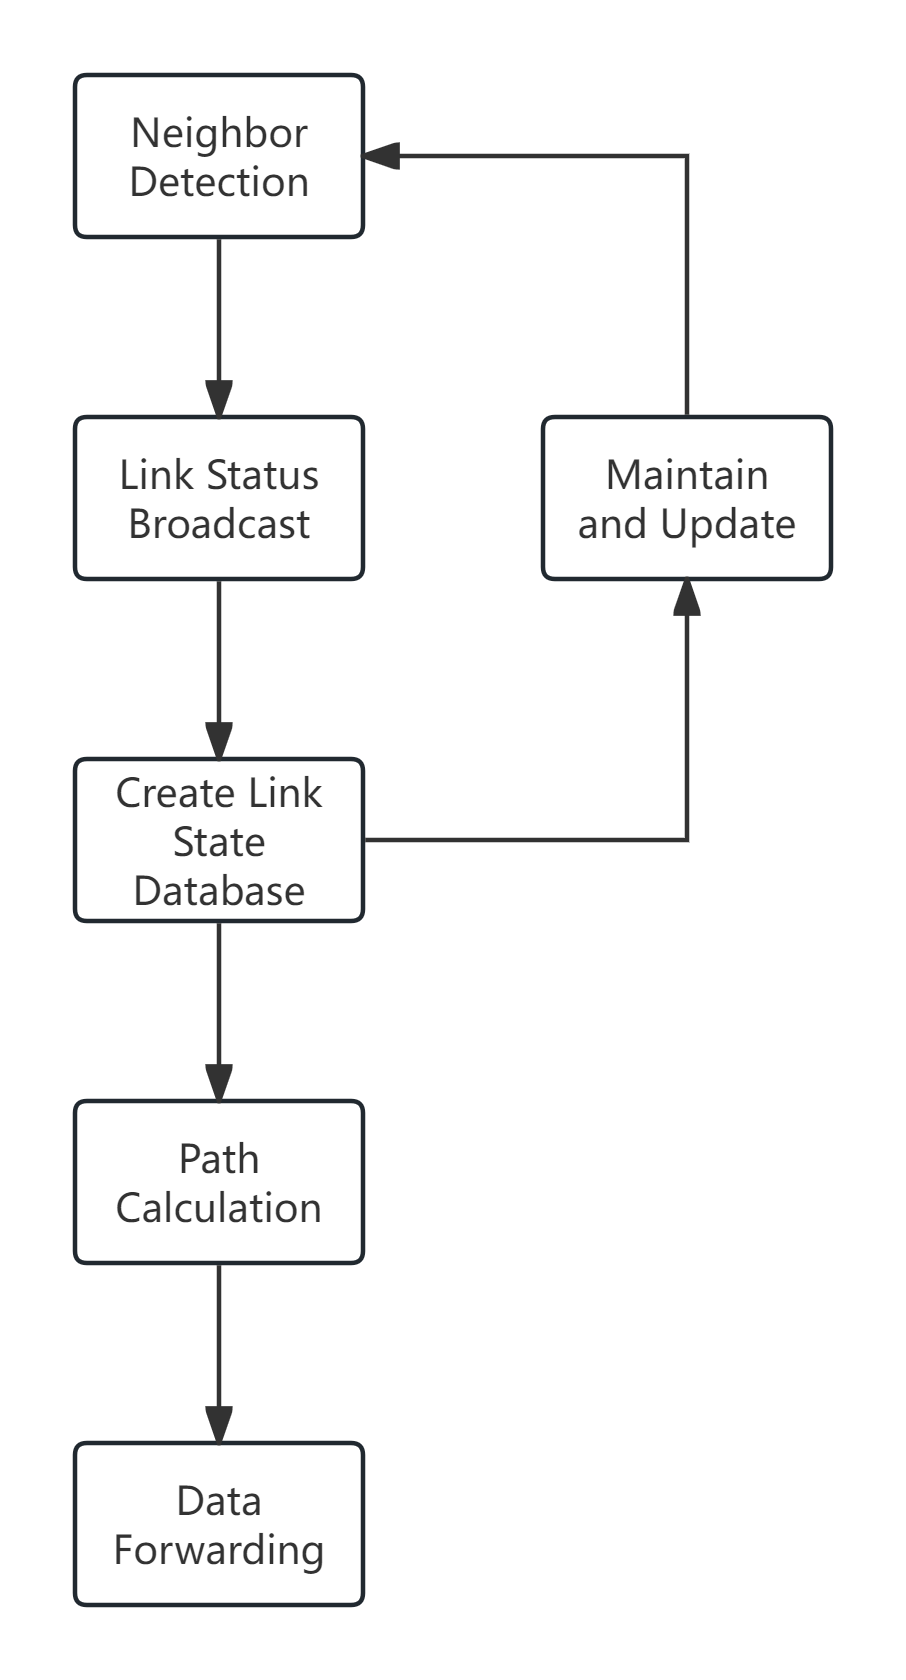
\includegraphics[width=0.5\linewidth]{figures/NLSR_Work_Flow.png}
    \caption{NLSR Work Flow}
    \label{fig:enter-label}
\end{figure}

\subsection{Producer Mobility Problems}
In NDN, the change in producer locations poses significant challenges to network communication. When a producer moves to a new location, it must re-register its data prefix in the network so that the forwarder can update the routing information to ensure the interest packets can be correctly forwarded to the new producer location. However, interest packets cannot find the new location of the producer until the routing information in the network is updated sufficiently to allow a new path to be built between the producer and the consumer. Therefore, after the producer moves, it needs to go through the process of routing update and consumer resending interest packets.

\begin{figure}
    \centering
    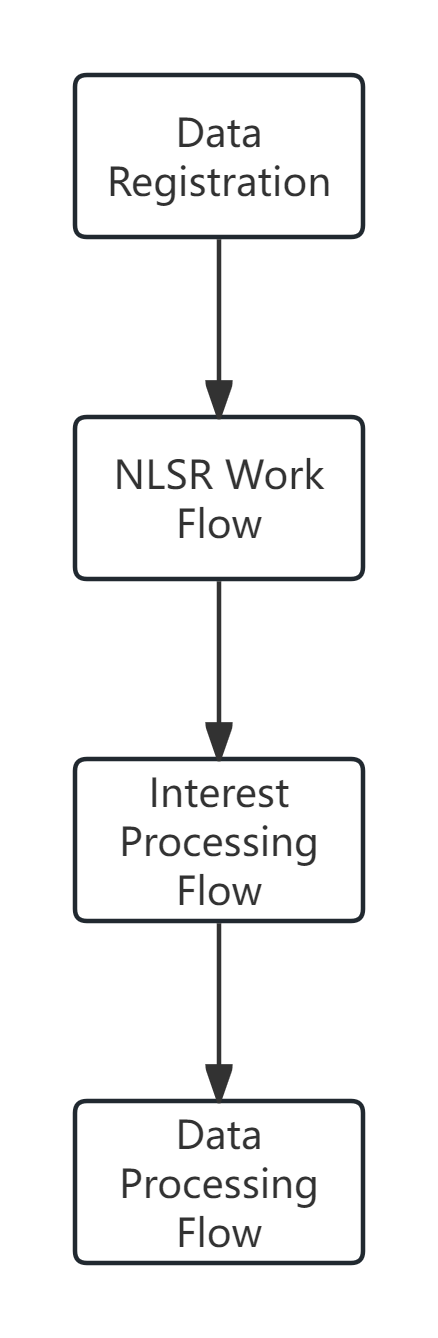
\includegraphics[width=0.5\linewidth]{figures/Producer_Mobility_Problems.png}
    \caption{Producer Mobility Problems}
    \label{fig:enter-label}
\end{figure}

The challenges introduced by producer mobility are reflected mainly in the following aspects.

\textbf{Latency:} When a producer moves, it takes time to re-register the data prefix and wait for the forwarder to update the routing information. Routing information updates are propagated gradually throughout the network, starting from the forwarder that the producer directly connects to. Therefore, until the routing information in the network is updated sufficiently to allow a new path to be built between the producer and the consumer, the communication between the producer and the consumer is interrupted. This results in a longer network response time. In a highly dynamic network environment where producers move frequently, such delays can accumulate, significantly degrading the quality of communication.

\textbf{Packet Loss:} From the the producer changes its location to the necessary routing updates are completed, interest packets sent by the consumer cannot reach the new location of the producer, resulting in data request failure and interest packets being discarded. In addition, the interest packets that the producer received but did not respond to before the move, the corresponding data packets can be sent to the newly connected node. However, if the node is not on the path that the interest packet previously passed on, its PIT will not store the return path of the data packet. The data packet will wait on the node until its life cycle is exhausted and then abandoned. This will increase the data packet loss rate and weaken the reliability of data transmission.

\textbf{Network Resource Usage:} Network resource usage is a critical performance metric. The issues caused by packet loss and retransmissions due to producer mobility can lead to additional resource consumption. Furthermore, any solution designed to address producer mobility should prevent significantly increasing network resource usage. Otherwise, they may negatively impact other communications on the network.

In general, producer mobility introduces challenges such as increased latency, packet loss, and increased resource consumption in NDN. These issues are particularly prominent in highly dynamic network environments, necessitating effective solutions to optimise network performance.

\section{Controllable Flooding for NDN Mobility}
To address the challenges of producer mobility in NDN, we propose a controllable flooding mechanism for data packets. This mechanism reduces the reliance on routing updates by optimising the propagation of data packets after a producer moves. The purpose is to reduce the impact of producer mobility on network communications, especially in application scenarios such as live streaming that have high requirements for network communication quality.

\subsection{Data Packet Flooding Mechanism}
From a practical perspective, producers in mobile scenarios usually move between adjacent nodes rather than instantly jumping to distant, non-adjacent nodes. This behaviour allows the new node where the producer reconnects to flood previously received but unanswered data packets to nodes along the previous path. These nodes typically maintain a valid path to the consumer requesting the data, allowing the return of data packets to the consumer without waiting for routing updates.

To implement this, we modified the structure of the NDN data packet by adding a \textit{MobilityFlag} field in the \textit{MetaInfo} section. This field indicates whether the data packet originates from a mobile producer. When a producer detects a change in its network interface (for example, disconnection or switching), it sets the \textit{MobilityFlag} and generates data packets for any pending interest packets received before the move. The data packets are then flooded to the neighbouring nodes.

Upon receiving a data packet with the \textit{MobilityFlag}, a forwarder temporarily overrides the standard routing rules. Instead of forwarding the packet according to its PIT, the forwarder propagates the packet to all its neighbours. If the flooded packet eventually reaches a node whose PIT contains the corresponding interest, the forwarder removes the \textit{MobilityFlag} and routes the packet normally to the consumer.

This mechanism eliminates the need for nodes along the path to wait for global routing updates or for the consumer to re-send the same interest packets. As a result, it significantly reduces the delay caused by producer mobility and ensures that interest packets received before the move are processed properly. However, this approach is most effective in scenarios where producers move within a unified network, such as between base stations in a cellular network or between access points in a WiFi network.

\subsection{Implementation of the Flooding Mechanism}
The implementation of the flooding mechanism involves two key components: modifications to the producer's behaviour and changes in the forwarder's packet processing logic.
\subsubsection{Producer Behaviour and Data Packet Extension}
The producer can detect changes in its network interface, such as a switch between access points or a disconnect. Upon detecting mobility, the producer marks the \textit{MobilityFlag} field in the \textit{MetaInfo} section of the NDN data packet. This modification is a lightweight extension to the existing protocol and does not affect its core logic. The producer iterates through its pending interest packets, generates corresponding data packets, and sends them upon reconnecting to a new node.
\subsubsection{Forwarder Logic for Flooding}
Upon receiving a packet with \textit{MobilityFlag}, the forwarder checks its PIT for a matching interest. If no match is found, the forwarder propagates the packet to all its neighbouring nodes instead of forwarding it using the FIB. If a match is found in the PIT, indicating that the flooded packet has reached the target, the forwarder removes the \textit{MobilityFlag} and resumes normal routing for the packet. To avoid excessive resource consumption, floods are controlled by setting limits on the propagation scope, such as a maximum number of hops.

\subsection{Flooding Control Mechanism}
To optimise the use of network resources and prevent uncontrolled flooding, we propose a fine-grained flood control mechanism. This mechanism introduces dual restrictions—hop count limits and time constraints—on the propagation of flooded packets.
\subsubsection{Flooding Control Indicators}
To achieve controlled flooding, two additional fields—\textit{HopLimit} and \textit{Timestamp}—are added to the \textit{MetaInfo} section of packets with the \textit{MobilityFlag}. These fields guide the propagation of flooded packets.

\textit{HopLimit}: This field specifies the maximum number of hops that a flooded packet can traverse. Each time a forwarder receives and forwards a packet, it decreases the \textit{HopLimit} by 1. Once the value reaches 0, the forwarder discards the packet and stops further propagation.

\textit{Timestamp}: This field records the time when the packet is generated. The forwarder uses this timestamp to ensure that the total lifetime of the packet does not exceed a predefined maximum TTL (for example, 5 seconds). If the difference between the current time and the packet's timestamp exceeds the TTL, the packet is discarded.

These dual restrictions ensure that flooding behaviour is strictly controlled, preventing unnecessary resource consumption and limiting the impact on the network.

\subsubsection{Forwarder Behaviour for Flooding Control}
When a forwarder processes a packet with the \textit{MobilityFlag}, it follows a specific logic to manage flooding:

\textit{HopLimit} Check: The forwarder checks the \textit{HopLimit} field. If the value is greater than 0, the packet is forwarded to the neighbouring nodes with \textit{HopLimit} decremented by 1. If the value is 0, the packet is discarded.

TTL Verification: The forwarder compares the \textit{Timestamp} of the packet with the current time. If the elapsed time exceeds the TTL, the packet is discarded.

Interest Packet Match: If the packet matches an interest stored in the forwarder’s PIT, it indicates that the forwarder is part of the pre-move path. In this case, the forwarder removes the \textit{MobilityFlag} from the packet and allows it to propagate normally within the network, unrestricted by \textit{HopLimit} or TTL.

By combining these flood control measures, our solution reduces delays and packet loss while efficiently managing network resources. This ensures optimal performance for NDN in dynamic environments.

\section{Experiment}
\subsection{Experimental Design}
This experiment evaluates the performance comparison between the traditional global route update mechanism and controllable flooding technology in NDN when facing producer mobility problems. By simulating video transmission, this experiment examines in detail the ability of both mechanisms to handle real-time data streams under dynamic network conditions, especially in transmission delay, packet loss rate, and network load.

The reason for choosing video transmission as the experimental scenario is that the continuity and integrity of video content are crucial to user experience, and its high demand for real-time performance can effectively demonstrate network performance differences. Meanwhile, mobile video transmission scenarios are common in the real world, such as users conducting video meetings and online live streams on vehicles, where quickly and effectively adapting to changes in producer locations is the key to maintaining service quality.

Therefore, this experiment provides quantitative data on the performance changes after implementing the new technology and demonstrates its application potential and practical benefits under high load and dynamically changing conditions.

\subsubsection{Consumer Application}
The consumer application is designed to automatically request, receive, and process data packets at a high frequency to ensure the real-time and sequential nature of the data. The program is specifically designed to simulate data stream processing in real-time video applications. The specific implementation details are as follows:

Automatic data request: The consumer program automatically sends interest packets, each of which has a predefined prefix, such as /example/livestream/, and a version number is attached to identify different data requests. The interest packets are set to be the latest and have a life cycle of 6 seconds to ensure the timeliness of the request.

Request frequency: In order to meet the high packet transmission frequency requirements of real-time video transmission, the consumer sends a new interest packet every 33 milliseconds. This setting is based on the need to simulate the transmission of 30fps video.

Management and retransmission of unresponsive interest packets: The consumer application introduces an unresponsive interest packet queue to store interest packets that have not responded due to timeout. The unresponsive queue uses a first-in-first-out (FIFO) strategy. When the queue is full, the earliest interest packet will be discarded to make room. Unresponsive interest packets will not be retransmitted at the normal sending frequency, but will be sent at a uniform retransmission frequency of once per second to ensure low occupancy of network resources.

Data reception and verification: After receiving the data, the consumer outputs the data content and verifies the authenticity of the data using the preloaded trust architecture configuration. When the data packet conforms to the trust architecture, the system outputs confirmation information; if the verification fails, the verification error is reported.

Error handling: If a NACK (negative acknowledgement) packet is received, the consumer outputs the NACK reason. If the interest packet times out without a response, the timeout information is output and the interest packet is resent in the next cycle.

Naming rules and data integrity: The name of the data packet requested by the consumer follows the predefined naming rules to ensure that the received data packet conforms to the expected naming rules, thereby ensuring the integrity and correctness of the data.

The consumer program ensures the real-time and reliability of data stream processing through a reasonable interest packet sending frequency and an effective error handling mechanism, which is suitable for the simulation environment of real-time video transmission.

\subsubsection{Producer Application}
The producer application plays a vital role in the video transmission system, responsible for processing and publishing data to consumers. The program is designed to simulate real-time video transmission and ensure smooth transmission by responding to the data packets requested by the producer in a timely manner. The specific tasks and implementation details are as follows:

Prefix registration: The producer program registers the prefix /example/testApp through the system call automatic advertisement to ensure that the interest packet request for the prefix can be received. This registration process is completed by calling the nlsrc advertise command.

Interest packet processing: The producer application listens for interest packet requests with a specific prefix by setting interest packet filters. When receiving an interest packet request from a consumer, the producer generates a data packet matching the request name. The data packet is set to a freshness period of 10 seconds to ensure the timeliness of the data.

Data content generation and signing: Whenever an interest request from a consumer is received, the producer generates a packet containing the corresponding content. In this implementation, the content of the data packet is a simple string "Hello, world!". Then, the data packet is signed using the default key chain to ensure its integrity and security.

Mobility flag and data packet flooding: When the producer detects a change in the network interface (such as disconnection or switching), the producer will add a MobilityFlag tag to the data packet generated in response to the interest packet to indicate its mobility status. At the same time, these data packets will be attached with a hop limit (HopLimit) and a timestamp to control the flooding range and time. When the data packet reaches the forwarder, the data packet carrying the MobilityFlag will be propagated to all neighboring nodes according to the flooding mechanism instead of following the traditional routing rules.

Data packet sending: After the signature is completed, the producer sends the data packet back to the requested consumer. This process ensures that consumers can receive complete and verified data responses.

Naming rules: The producer application uses a clear naming convention to identify data packets. The name of each data packet is based on the name of the consumer interest packet. For example, if the name of the data packet requested by the consumer is //example/livestream/1, the producer will generate a data packet with this name and return it to the consumer. This naming convention ensures the accuracy of the request and the availability of the data packet.

Error handling: If the prefix registration fails, the producer will output an error message and close the connection with the forwarder to avoid continuing to receive interest packet requests that cannot be processed.

The producer program ensures the real-time and reliability of data stream processing through an effective interest packet processing and data packet generation mechanism, which is suitable for the simulation environment of real-time video transmission.

\subsubsection{Network Topology}
The experiment was constructed using a classic three-layer mobile network model, including:
\begin{itemize}
    \item Core layer: 1 core layer switch.
    \item Distribution layer: 2 aggregation layer switches, each connected to the core layer switch.
    \item Access layer: Each aggregation layer switch is connected to 3 access layer switches.
    \item Core-to-distribution connection: 1 Gbps bandwidth, 1 ms latency.
    \item Distribution-to-access connection: 1 Gbps bandwidth, 1 ms latency.
    \item Access-to-client connection: 100 Mbps bandwidth, 10 ms latency.
\end{itemize}

\begin{figure}
    \centering
    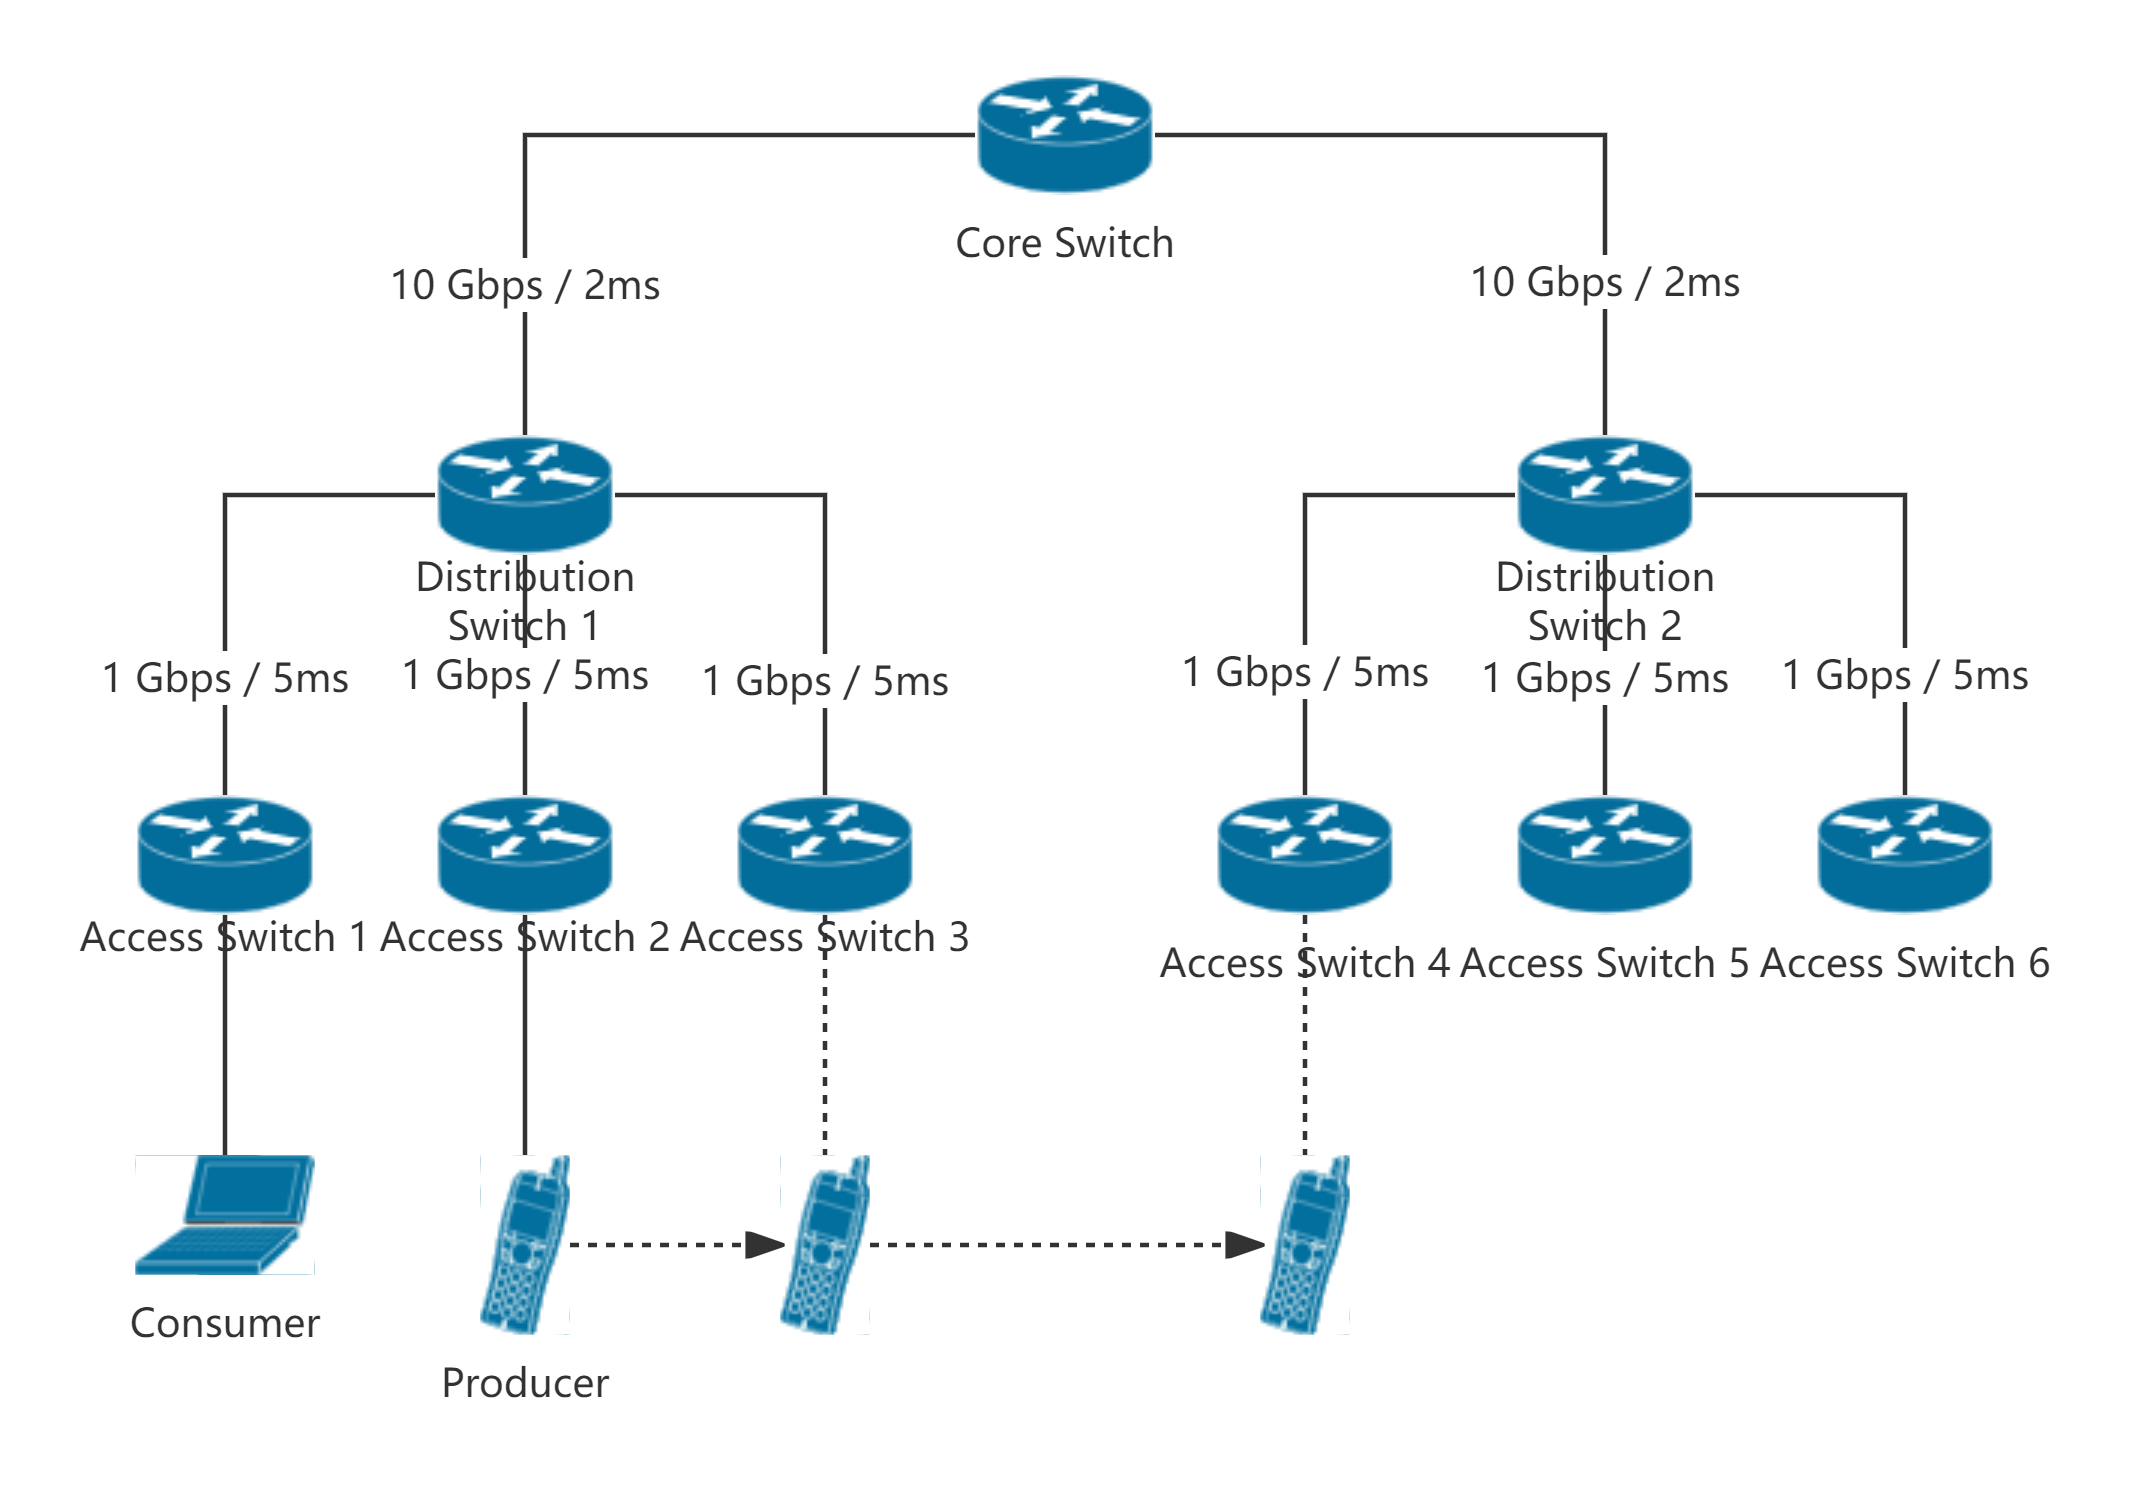
\includegraphics[width=\columnwidth]{figures/Topology.png}
    \caption{Experiment}
    \label{fig:enter-label}
\end{figure}

\subsection{Baseline Test}
This experiment aims to evaluate the impact of producer mobility in NDN on video transmission performance, especially when the new mechanism (controlled flooding) is not enabled. The experiment measures the impact of producer mobility in the network topology on latency, packet loss rate, and network response time. The experiment is conducted in the Mini-NDN simulation environment, with consumer and producer applications running on designated nodes respectively.

First, start the Mini-NDN environment and initialize all network nodes. During the startup process, NFD and NLSR are started on all nodes. In this step, wait for the NLSR protocol to start and reach a stable state, which can usually be achieved within 20 seconds to ensure that the network routing information is correctly propagated and stable.

After the network configuration is completed, start the tcpdump tool on the consumer node to listen and capture packets in the network and save them as consumer\_capture.pcap file for subsequent analysis. This step provides a detailed record of network communication during the experiment, which can help accurately analyze the impact of producer mobility on network performance.

Next, start the producer application on the producer node and the consumer application on the consumer node at the same time. The producer application is responsible for processing the interest packet request sent by the consumer and returning the corresponding data packet, while the consumer application periodically sends interest packets to request data. This process simulates the common data request and transmission behavior in real-time video streaming applications.

The core part of the experiment is to simulate the movement of the producer in the network. First, the producer is connected to the initial access switch (acc2). After a period of stable operation (30 seconds), the producer is moved from the initial access switch (acc2) to another access switch (acc3). This operation is achieved by disconnecting the producer from the current access switch and establishing a connection with the new access switch. After another 30 seconds of stable operation, the producer is moved again to another new access switch (acc4) to simulate multiple movements of the producer between different layers in the network. These movement operations are used to observe and measure the impact of producer movement on data transmission performance, including changes in transmission delay and packet loss rate.

After the experiment, stop data capture and terminate the tcpdump process, and then analyze the captured data file consumer\_capture.pcap to evaluate the specific impact of producer mobility on network performance. Finally, the operation status of the network can also be checked and verified through the command line interface of Mini-NDN to ensure the accuracy and reliability of the experimental results.

This experiment systematically simulates the movement of producers in the network and provides benchmark data for evaluating producer mobility issues in the NDN environment. These data will provide an important reference for subsequent research on the application effect of optimization mechanisms in producer mobility scenarios.

\begin{figure}
    \centering
    \includegraphics[width=\textwidth]{baseline_throughput.pdf} % Baseline 的结果文件
    \caption{Baseline Test Throughput}
    \label{fig:baseline-throughput}
\end{figure}

\subsection{Solution Test}
\begin{figure}
    \centering
    \includegraphics[width=\textwidth]{solution_throughput.pdf} % Solution 的结果文件
    \caption{Solution Test Throughput}
    \label{fig:solution-throughput}
\end{figure}

\subsection{Data Collection}
\begin{itemize}
    \item Intra-segment latency: Measures the time from when the producer sends each video segment to when the consumer receives it. This will help understand the impact of producer movement on individual packet transmission efficiency.
    \item Movement delay: Pay special attention to the additional delay caused when the producer's location changes. This can be evaluated by comparing the transmission latency of the same video clip before and after the producer moves between different access layer switches.
    \item Overall network response time: When the producer changes location and starts sending video data to when the consumer first receives the changed data. This metric captures how quickly the network responds to changes in producer location.
    \item Packet loss rate: The ratio of requested packets to successfully received packets.
    \item Network usage: The total bandwidth usage of the network during the experiment.
\end{itemize}

\section{Analysis}
This section will analyze in detail the performance of the controlled flooding mechanism in a dynamic network scenario. The analysis will be based on a simulated network environment, focusing on evaluating the improvement effect of the flooding mechanism on the producer mobility problem, including key performance indicators such as network latency, packet loss rate, and network resource utilization.

\subsection{Theoretical Analysis of Network Performance}
Delay reduction: It is expected that the delay of data transmission will be reduced by adopting the controlled flooding mechanism. Since packets can be propagated immediately without waiting for global routing updates, the data transmission time after the producer's location changes should be faster than the traditional global routing update mechanism.

Packet loss rate: In a dynamic network environment, especially in scenarios where producers move frequently, traditional routing update methods may result in high packet loss rates. The controlled flooding mechanism reduces such problems by quickly responding to location changes, thereby improving the reliability of data transmission.

Network load management: Although the flooding mechanism may increase the initial network load, the occupation of network resources can be effectively controlled through appropriate control strategies, such as hop limit and packet life cycle management, thereby optimizing the overall network performance.

\subsection{Discussion of expected results}
Based on the above theoretical analysis, we can predict that the controlled flooding mechanism performs well in reducing latency and improving data transmission reliability. In addition, although the network resource utilization may increase in the early stage of the experiment, in the long run, the overall resource efficiency of the network should be improved.

\section{Related Work}
\todo{compare our results with some related works, to prove that our solution is better.}
Many scholars have proposed different solutions to the producer mobility problem in past research. For example, Zhang et al. proposed a tunnel-based solution that allows interest packets to be sent directly to moved producers while fully utilizing the caching function of NDN using a specific naming scheme. This solution effectively reduces network costs and optimizes routing (Zhang et al., 2017). In addition, Abrar et al. developed a mechanism to improve the NDN forwarding plane to support mobile data packets, solving problems such as interest packet loss and non-optimal routing paths when producers move (Abrar et al., 2022). The ProCacheMob scheme introduced by Farahat and Hassanein effectively reduces delays and packet loss during producer movement by predicting future interests and caching data before handover (Farahat \& Hassanein, 2017).

Although these studies have made some progress in dealing with producer mobility, they still leave much space to explore. Existing research on data flooding in NDN mainly focuses on network security issues, such as detecting and defending interest flooding attacks (Tang et al., 2013). It has yet to attempt to use the flooding mechanism to solve the producer mobility problem.

This solution sends data packets directly to the forwarder after the producer moves and allows the forwarder to flood the data packets to neighbour nodes that may have a return path. This method can effectively handle the producer mobility problem in practical applications, filling the gap in existing research.

\csp{add discussion of Cullen Jennings' MoQ work, which has a very NDN flavour}

\section{Conclusion and Future Work}
\subsection{Conclusion}
WORKING IN PROGRESS...
\subsection{Long Term Impact Assessment}
\subsubsection{Continuous optimization of network performance}
\begin{itemize}
    \item Efficiency Improvements: Long-term application of this strategy may lead to continued improvements in the network's overall efficiency, especially in data transfer speeds and reduced latency.
    \item Enhanced Reliability: The network may gradually adapt to new propagation mechanisms over time, improving overall data transmission reliability.
\end{itemize}

\subsubsection{Resource Usage and Network Stability}
\begin{itemize}
    \item Resource Optimization: Long-term implementation may lead to more efficient use of network resources, especially regarding packet propagation and drop strategies.
    \item Stability Analysis: Evaluate the impact of this strategy on network stability over time, especially in the face of high loads and dynamic changes.
\end{itemize}

\subsection{Future Development Direction}
Discuss how this strategy can be further optimized to adapt to changes in the future network environment as technology develops. Consider possible future application scenarios of this strategy, such as the Internet of Things, smart cities, etc.


\section*{Acknowledgment}

The preferred spelling of the word ``acknowledgment'' in America is without 
an ``e'' after the ``g''. Avoid the stilted expression ``one of us (R. B. 
G.) thanks $\ldots$''. Instead, try ``R. B. G. thanks$\ldots$''. Put sponsor 
acknowledgments in the unnumbered footnote on the first page.

\section*{References}

Please number citations consecutively within brackets \cite{b1}. The 
sentence punctuation follows the bracket \cite{b2}. Refer simply to the reference 
number, as in \cite{b3}---do not use ``Ref. \cite{b3}'' or ``reference \cite{b3}'' except at 
the beginning of a sentence: ``Reference \cite{b3} was the first $\ldots$''

Number footnotes separately in superscripts. Place the actual footnote at 
the bottom of the column in which it was cited. Do not put footnotes in the 
abstract or reference list. Use letters for table footnotes.

Unless there are six authors or more give all authors' names; do not use 
``et al.''. Papers that have not been published, even if they have been 
submitted for publication, should be cited as ``unpublished'' \cite{b4}. Papers 
that have been accepted for publication should be cited as ``in press'' \cite{b5}. 
Capitalize only the first word in a paper title, except for proper nouns and 
element symbols.

For papers published in translation journals, please give the English 
citation first, followed by the original foreign-language citation \cite{b6}.

\begin{thebibliography}{00}
\bibitem{b1} G. Eason, B. Noble, and I. N. Sneddon, ``On certain integrals of Lipschitz-Hankel type involving products of Bessel functions,'' Phil. Trans. Roy. Soc. London, vol. A247, pp. 529--551, April 1955.
\bibitem{b2} J. Clerk Maxwell, A Treatise on Electricity and Magnetism, 3rd ed., vol. 2. Oxford: Clarendon, 1892, pp.68--73.
\bibitem{b3} I. S. Jacobs and C. P. Bean, ``Fine particles, thin films and exchange anisotropy,'' in Magnetism, vol. III, G. T. Rado and H. Suhl, Eds. New York: Academic, 1963, pp. 271--350.
\bibitem{b4} K. Elissa, ``Title of paper if known,'' unpublished.
\bibitem{b5} R. Nicole, ``Title of paper with only first word capitalized,'' J. Name Stand. Abbrev., in press.
\bibitem{b6} Y. Yorozu, M. Hirano, K. Oka, and Y. Tagawa, ``Electron spectroscopy studies on magneto-optical media and plastic substrate interface,'' IEEE Transl. J. Magn. Japan, vol. 2, pp. 740--741, August 1987 [Digests 9th Annual Conf. Magnetics Japan, p. 301, 1982].
\bibitem{b7} M. Young, The Technical Writer's Handbook. Mill Valley, CA: University Science, 1989.
\end{thebibliography}
\end{document}
